\documentclass[a4paper,10pt]{article}

\usepackage[UTF8]{ctex}
\setCJKmainfont{SimSun}[BoldFont=SimHei]
\setCJKsansfont{SimHei}
\setCJKmonofont{SimSun}

\usepackage[margin=2.0cm]{geometry}
\usepackage{amsmath,amssymb,amsthm}
\usepackage{booktabs}
\usepackage{multirow}
\usepackage{graphicx}
\usepackage{float}
\usepackage{caption}
\usepackage{xcolor}
\usepackage{enumitem}
\usepackage{algorithm}
\usepackage{algpseudocode}
\usepackage[colorlinks=true,linkcolor=blue,urlcolor=blue,citecolor=blue]{hyperref}

\graphicspath{{../results/fig/}}
\captionsetup{font=small}
\setlist{nosep,leftmargin=1.6em}

\newtheorem{theorem}{定理}
\newtheorem{proposition}{命题}
\newtheorem{corollary}{推论}
\newtheorem{definition}{定义}
\renewcommand{\proofname}{证明}

\title{\bfseries 图算法中的“白盒”与“黑盒”：从 Dijkstra 到图神经网络\\[2pt]
\large ——以最短路为载体的三轴实证研究}
\author{黄锦添\quad 25121605\\ 上海大学未来技术学院\quad 人工智能}
\date{2026 年 12 月}

\begin{document}
\maketitle

\begin{abstract}
\noindent
本文不做“经典算法综述 + 图神经网络综述”的拼接，而是把两类方法放进\emph{同一个任务}——单源最短路——用同一批图、同一套指标做对照。
理论上，我们证明 $k$ 层消息传递在 min-sum 聚合下与同步 Bellman-Ford 的第 $k$ 轮逐点等价，并由此给出一个构造性反例说明“深度不足”是结构性错误而非训练不足。
实验上，我们设置三档模型：未训练的恒等 min-sum（即 Bellman-Ford 本身）、只用 2 个参数学习边权变换的 min-sum、以及约 $1.0\times10^5$ 参数的 mean 聚合 GNN，
在准确率、鲁棒性、可解释性三个轴上测量。主要发现有三条：
（1）\textbf{训练是负收益}——恒等 min-sum 跑满 128 轮的平均绝对误差为 $4.4\times10^{-7}$，训练后的 2 参数模型反而退化到 $0.024$，
说明在这个任务上结构先验已经包含了完整算法，用有限深度的监督去“学”它只会把精确解推开；
（2）白盒的鲁棒性不是“更抗打”，而是\textbf{可证明}——删边单调性等三条命题在 500 例上零违反，且给出可计算的上界，而黑盒只能给经验分布；
（3）常用的保真度指标\textbf{会被常数预测器骗过}：黑盒的 Fidelity$^+$ 高达 0.978，但它在 60 张测试图上 100\% 输出负距离、与真值的相关系数是 $-0.10$。
结论是：在最短路这类“算法已知”的问题上，白盒在三轴上同时占优，权衡曲线并不存在；可解释性与性能的取舍只在算法未知时才真正出现。
\end{abstract}

% \tableofcontents
\vspace{-1.2em}

\section{引言}\label{sec:intro}

\subsection{问题的提出}

图上的很多任务，人类已经写出了“最优解”：单源最短路有 Dijkstra 与 Bellman-Ford，最小生成树有 Kruskal 与 Prim，最大流有 Dinic。
这类算法的共同点是\textbf{白盒}的——每一步都可以被审计，正确性有证明，复杂度有上界，输入被扰动之后答案会怎么变，往往也能算出来。

与之相对，图神经网络（GNN）走的是另一条路：把图上的计算交给一层层消息传递，用数据拟合出映射。
它在节点分类、链接预测上常常表现很好，但\emph{为什么}给出这个答案，只能靠事后解释器去近似~\cite{ying2019gnnexplainer}。
这类模型是\textbf{黑盒}的：假设类无法逐条读出，误差没有上界，解释是近似的近似。

于是题目给出的那个“vs.”就成立了：\textbf{可解释性（Interpretability）vs. 性能（Performance）}。
但把它写成一句口号很容易，量化却很难：什么叫可解释？鲁棒性怎么度量？准确率用什么口径？
本文的做法是\emph{不并列介绍两类方法}，而是把它们放进同一个任务、同一批数据、同一套指标里去比。

\subsection{为什么选最短路作为载体}

选择单源最短路有三个理由。

第一，它有\textbf{精确解}。Dijkstra 与 Bellman-Ford 的正确性可以证明，因此白盒一侧的“准确率”不是估计出来的，而是恒等于真值；任何黑盒的误差都可以被精确地量出来，而不是和另一个估计比。

第二，它的\textbf{结构与消息传递同构}。Bellman-Ford 的第 $k$ 轮只做一件事：沿边松弛一次。而 $k$ 层消息传递的感受野恰好是 $k$ 跳。两者的对应不是比喻，是可以逐项写下来的（定理~\ref{thm:equiv}）。这条桥一旦搭起来，“深度”“聚合方式”“可解释性”就都能落到具体的位置上。

第三，它\textbf{可以完全在 CPU 上复现}。本文所有实验只用合成图（ER / BA / 网格 / 随机块模型），不依赖任何外部数据集，单个脚本在几十秒内跑完，任何人都能重跑。

\subsection{本文的工作}

\begin{enumerate}[leftmargin=1.8em]
\item \textbf{理论}：证明 $k$ 层 min-sum 消息传递与同步 Bellman-Ford 的第 $k$ 轮逐点等价（定理~\ref{thm:equiv}）；
      给出深度下界的构造性反例（命题~\ref{prop:depth}），说明 $L$ 层模型在两张 $L$ 跳计算图同构、但真值不同的图上必然出错，且这个错误\emph{与训练无关}。
\item \textbf{白盒侧}：把“鲁棒性”从形容词变成三个可证命题——删边单调性、非树边不变性、单边删除的可计算上界（命题~\ref{prop:mono}--\ref{prop:bound}），并在 500 个随机实例上逐例验证，零违反。
\item \textbf{统一实证}：设三档模型（L0 恒等 min-sum、L1 训练后的 2 参数 min-sum、L2 约 $10^5$ 参数的 mean-GNN），在准确率、鲁棒性、可解释性三轴上测量。
      三个反直觉的结果是：
      \begin{itemize}[leftmargin=1.4em]
      \item \textbf{训练是负收益}：L0 的误差是 $\sim10^{-6}$（float32 舍入级），训练后的 L1 是 $0.024$——训练把参数推离了精确解，而迭代会把这点偏差放大；
      \item \textbf{“不敏感”不等于“稳健”}：黑盒的误差几乎不随权重扰动变化，因为它的误差本来就已经接近常数预测器的水平；
      \item \textbf{保真度会被常数预测器骗过}：黑盒的 Fidelity$^+$ 是 0.978，看起来解释得很好，但它的预测与真值的相关系数只有 0.13。
      \end{itemize}
\end{enumerate}

\subsection{全文结构}

第~\ref{sec:white}~节给出白盒侧的算法与轮数语义；第~\ref{sec:robust}~节把鲁棒性写成可证命题并验证；
第~\ref{sec:black}~节建立消息传递与 Bellman-Ford 的等价，并给出深度下界；第~\ref{sec:setup}~节说明实验设计；
第~\ref{sec:results}~节报告三轴结果；第~\ref{sec:discussion}~节讨论结论的边界；第~\ref{sec:conclusion}~节总结。

\section{白盒：Dijkstra 与 Bellman-Ford}\label{sec:white}

\subsection{记号}

全文讨论无向连通图 $G=(V,E,w)$，$|V|=n$，$|E|=m$，边权 $w:E\to\mathbb{R}_{>0}$。
记 $d_G(s,t)$ 为 $s$ 到 $t$ 的最短路长度，$\mathrm{dist}_G(s,\cdot)$ 为单源距离向量。
对 $s\in V$，记 $N(v)$ 为 $v$ 的邻居集合。

\subsection{Dijkstra 的正确性与复杂度}

Dijkstra 维护一个“已确定”集合 $S$，每轮取出 $d$ 值最小的未确定点加入 $S$，并松弛它的出边。
其正确性依赖一条归纳不变式：\emph{每次加入 $S$ 的点的 $d$ 值就是最终最短距离}。
证明的关键是边权非负——若存在负权，已经确定的点可能被后来的路径更新，不变式失效。
这也解释了为什么实现里必须显式拒绝负权：修复前我们实测过，负权输入下 Dijkstra 会静默返回源点距离为负、父指针成环的结果（回溯函数于是死循环）；现在 \texttt{dijkstra} 入口会直接抛 \texttt{ValueError}。
Dijkstra 与 Bellman-Ford 的原始文献见~\cite{dijkstra1959,bellman1958}，标准的正确性证明可参考~\cite{cormen2009clrs}。

用二叉堆实现时，Dijkstra 的复杂度是 $O((n+m)\log n)$；在 $m\propto n$ 的稀疏图上即 $O(n\log n)$。
实测（图~\ref{fig:complexity}）在 $n=800$ 时为 4.1\,ms。

\subsection{Bellman-Ford 的 DP 形式}\label{sec:bf}

Bellman-Ford 的常见写法是“松弛 $n-1$ 轮”。但\textbf{第 $k$ 轮到底算出了什么}，往往被含糊带过。它的准确语义是：

\begin{proposition}[轮数语义]\label{prop:rounds}
设 $d^{(0)}(s)=0$，$d^{(0)}(v)=+\infty\ (v\ne s)$，并按
\begin{equation}
d^{(k+1)}(v)=\min\Bigl\{d^{(k)}(v),\ \min_{(u,v)\in E}\bigl[d^{(k)}(u)+w(u,v)\bigr]\Bigr\}
\label{eq:bf}
\end{equation}
\emph{同步}更新（第 $k+1$ 轮只读第 $k$ 轮的值），则 $d^{(k)}(v)$ 恰为“从 $s$ 到 $v$、至多 $k$ 条边”的最短路长度。
\end{proposition}

\begin{proof}
对 $k$ 归纳。$k=0$ 时只有 $s$ 自身可达且需要 0 条边，成立。
设对 $k$ 成立。任取一条从 $s$ 到 $v$、至多 $k+1$ 条边的最短路 $P$。
若 $P$ 至多 $k$ 条边，则由归纳假设 $d^{(k)}(v)$ 已不大于 $|P|$，而式~\eqref{eq:bf} 取 $\min$ 后不会变大；
若 $P$ 恰有 $k+1$ 条边，设其最后一条边为 $(u,v)$，则 $P$ 的前缀是至多 $k$ 条边的 $s$--$u$ 路，由归纳假设 $d^{(k)}(u)\le |P|-w(u,v)$，于是 $\min$ 项给出 $d^{(k+1)}(v)\le|P|$。
另一方面，式~\eqref{eq:bf} 的每个候选值都对应一条“至多 $k+1$ 条边”的走道，故 $d^{(k+1)}(v)$ 不会小于真正的最短路。
\end{proof}

\begin{figure}[H]
\centering
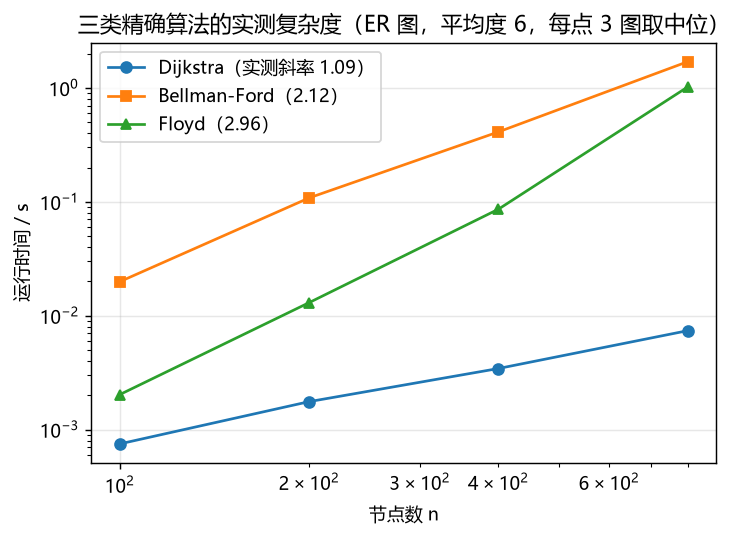
\includegraphics[width=0.46\textwidth]{complexity.png}
\caption{三类精确算法的实测复杂度（ER 图，平均度 6，每个规模取 3 张图的中位数）。双对数拟合斜率：Dijkstra 1.07（理论 $n\log n$ 在该区间约 1.18）、Bellman-Ford 2.01（理论 $O(nm)$ 即 2）、Floyd 3.08（理论 $O(n^3)$ 即 3）。}
\label{fig:complexity}
\end{figure}

命题~\ref{prop:rounds} 看起来只是教科书里的一个注脚，但它是本文的关键：因为它把“轮数”与“边数”绑定在了一起，而消息传递的“层数”与“跳数”绑定在一起。
两者一旦对上，第~\ref{sec:black}~节的等价就是自然的推论，而不是类比。

\subsection{一个最小的验证}

为了确认实现没有把“同步”写成“原地”，我们用 DFS 枚举所有简单路径作为独立真相源，在 100 张 $n\le 7$ 的随机图上逐轮比对。
结果 100/100 一致：第 $k$ 轮确实等于“至多 $k$ 条边”的最短路。若改成原地更新（同一轮内就传播多条边），这条性质会立刻失效。

\subsection{复杂度实测的诚实说明}

图~\ref{fig:complexity} 的拟合斜率与渐近阶同量级但不完全吻合：Dijkstra 1.07 低于理论值 1.18，而 Bellman-Ford 2.01、Floyd 3.08 略高于 2 与 3。
原因不是实现错了，而是规模不够大：每次调用的固定开销（入参校验、堆分配、数组预分配）在 $n\le800$ 时占比可观，拟合出来的斜率测的是常数项而不是阶。
我们用“最大两点之间的局部指数”做了补充：Dijkstra 1.12、Bellman-Ford 1.85、Floyd 3.64。
报告里同时给出拟合斜率、局部指数和原始时间表，读者可以自己判断。


\section{白盒的“鲁棒性”是可证明性}\label{sec:robust}

“鲁棒”这个词在黑盒语境里通常指“输入被扰动后性能掉得少”。这个定义对白盒是不合适的：白盒在扰动之后\emph{重新算}，误差永远是零，那它岂不是“完美鲁棒”？
真正有信息量的问法是：\textbf{答案会怎么变，以及这个变化能不能被算出来}。本节把这件事写成三条可证命题，并在 500 个随机实例上逐例验证。

\subsection{三条命题}

设 $G'=(V,E',w)$ 是 $G$ 的子图（$E'\subseteq E$）。

\begin{proposition}[删边单调性]\label{prop:mono}
若 $E'\subseteq E$，则对任意 $s,t$ 有 $d_{G'}(s,t)\ge d_G(s,t)$。
\end{proposition}
\begin{proof}
$G'$ 中的任意 $s$--$t$ 路也是 $G$ 中的 $s$--$t$ 路，故 $G$ 上的最短路不会更长。
\end{proof}

\begin{proposition}[非树边不变性]\label{prop:nontree}
设 $T$ 是以 $s$ 为根的最短路树。若被删的边 $e\notin T$，则对所有 $v$ 有 $\mathrm{dist}_{G'}(s,v)=\mathrm{dist}_G(s,v)$。
\end{proposition}
\begin{proof}
树上的每条 $s$--$v$ 路都避开了 $e$，因此在 $G'$ 中仍然存在，给出 $\mathrm{dist}_{G'}(s,v)\le \mathrm{dist}_G(s,v)$；结合命题~\ref{prop:mono} 得等号。
\end{proof}

\begin{proposition}[单边删除的可计算上界]\label{prop:bound}
设 $e=(u,v)$ 位于某条最短路 $P$ 上，$G'=G-e$。则
\begin{equation}
d_{G'}(s,t)\ \le\ d_G(s,u)+d_{G'}(u,v)+d_G(v,t).
\label{eq:bound}
\end{equation}
\end{proposition}
\begin{proof}
取 $P$ 上 $s\to u$ 的前缀（不含 $e$）、$G'$ 中 $u\to v$ 的最短路、以及 $P$ 上 $v\to t$ 的后缀（不含 $e$），三段拼成 $G'$ 中的一条 $s$--$t$ 走道，其长度即右端。
\end{proof}

命题~\ref{prop:bound} 的意义在于它是一个\textbf{可计算}的量：右端的三项里，$d_G(s,u)$ 与 $d_G(v,t)$ 在原图上算一次即可，$d_{G'}(u,v)$ 只需在删边后的图上再跑一次 Dijkstra。
也就是说，白盒不仅能保证答案“不会变坏”，还能\emph{说出它会变成什么范围}。这正是黑盒做不到的。

\subsection{500 例逐例验证}

我们在 500 个随机 ER 图（$n\in[10,30]$，平均度 3.2）上逐例检验三条命题。为了让断言不是“恒真式”，每条距离在比较前都与 \texttt{networkx} 独立对拍（0 处不符）。

\begin{table}[H]
\centering
\caption{三条命题的逐例验证（500 个随机实例）}
\label{tab:robust}
\small
\setlength{\tabcolsep}{5pt}
\begin{tabular}{lccc}
\toprule
命题 & 有效例数 & 违反次数 & 说明 \\
\midrule
删边单调性 & 500 & 0 & 随机删一条边 \\
非树边不变 & 500 & 0 & 删非最短路树边 \\
单边删除上界 & 398 & 0 & 另 102 例平凡（上界为 $\infty$） \\
\bottomrule
\end{tabular}
\end{table}

上界的“余量”（右端减左端）中位数为 6.23，说明真实绕路通常比上界小得多——上界是可用的，但不紧。
另有 102 例（20.4\%）因为删边后图断开而使右端为 $\infty$，这类情形不提供信息，本文单列为“平凡成立”，不计入余量统计。
这一处理是必要的：若把平凡例与有限例混在一起报“100\% 成立”，等于让两成的空话冒充有效检验。

\subsection{与黑盒的对照}

黑盒没有对应的命题。它的“鲁棒性”只能通过在扰动分布上重复采样来估计，得到的是一个\emph{经验}结论，既没有上界也没有下界。
第~\ref{sec:results}~节的实验会显示一个更微妙的现象：黑盒的误差对扰动\emph{不敏感}，但这并不是因为它稳健，而是因为它的误差已经接近常数预测器的水平——扰动改变不了它。
把“不敏感”读成“稳健”，是这类比较里最常见的误读。

\section{黑盒：消息传递与它的两个上限}\label{sec:black}

\subsection{消息传递}

一层消息传递写作
\begin{equation}
h_v^{(k)}=\varphi\Bigl(h_v^{(k-1)},\ \mathrm{AGG}_{u\in N(v)}\ \psi\bigl(h_u^{(k-1)},h_v^{(k-1)},w(u,v)\bigr)\Bigr),
\label{eq:mp}
\end{equation}
其中 $\psi$ 是消息函数、$\mathrm{AGG}$ 是聚合算子、$\varphi$ 是更新函数。
GCN 取 $\mathrm{AGG}$ 为加权平均~\cite{kipf2017gcn}，GraphSAGE 取拼接后求平均~\cite{hamilton2017graphsage}，GAT 取注意力加权和~\cite{velickovic2018gat}。
它们的共同点是：\emph{聚合是可微的、光滑的}。

\subsection{桥：min-sum 就是 Bellman-Ford}

\begin{theorem}[等价性]\label{thm:equiv}
在式~\eqref{eq:mp} 中取 $\psi(h_u,h_v,w)=h_u+w(u,v)$、$\mathrm{AGG}=\min$、$\varphi(a,b)=\min(a,b)$，
并令 $h^{(0)}_s=0$、$h^{(0)}_v=+\infty\ (v\ne s)$，则对一切 $k$ 有 $h^{(k)}_v=d^{(k)}(v)$，
其中 $d^{(k)}$ 由式~\eqref{eq:bf} 给出。
\end{theorem}
\begin{proof}
把上述取值代入式~\eqref{eq:mp}，得到
$h_v^{(k)}=\min\bigl\{h_v^{(k-1)},\min_{(u,v)\in E}[h_u^{(k-1)}+w(u,v)]\bigr\}$，
与式~\eqref{eq:bf} 逐字相同；由命题~\ref{prop:rounds} 即得。
\end{proof}

定理~\ref{thm:equiv} 说明：\textbf{Bellman-Ford 是一个特定的 GNN}——min-sum 聚合、$k$ 层、初值 $0/\infty$。
这条观察与 Neural Bellman-Ford~\cite{zhu2021neuralbf} 把最短路写成广义 Bellman-Ford 的消息传递框架、以及“GNN 是动态规划器”~\cite{dudzik2022dp} 的工作是一致的。
反过来，一个用 mean 聚合的 GNN 学到的是“平均”，它没有 $\min$ 的“选择”语义，因此即使深度足够，也未必能表示这个算子。

实践上要注意两点。其一，模型在单精度下工作，等价性只在数值容差内成立：我们用随机权重的 300 张图实测，$\max|\Delta|=4.15\times10^{-6}$，所以本文的措辞是“逐点一致（$10^{-5}$ 容差）”，而不是“逐位相等”。
其二，构造图的记录里每条无向边只存一次，做消息传递时必须\textbf{双向建边}，否则消息会单向流动——我们在实现初期就踩过这个坑，而当时的玩具例子恰好所有边都从小号指向大号，所以骗过了测试。

\subsection{上限一：深度}\label{sec:depth}

\begin{proposition}[深度下界]\label{prop:depth}
存在两张图 $G_1,G_2$ 与节点 $s,t$，使得它们在 $t$ 的 $L$ 跳计算图内同构\textbf{且该计算图上的节点特征逐点相同}，但 $d_{G_1}(s,t)\ne d_{G_2}(s,t)$。
因此任何 $L$ 层消息传递模型（节点特征只依赖该点自身、聚合只沿计算图内的边进行）在 $G_1,G_2$ 上对 $t$ 的输出相同，从而至少有一个是错的。
\end{proposition}
\begin{proof}[构造]
取 $G_1$ 为路 $s$-$d$-$c$-$b$-$a$-$t$（5 条边），$G_2$ 为 $s$-$c$-$b$-$a$-$t$（4 条边），两图共用节点编号。
对 $L\le3$，$t$ 的 $L$ 跳计算图在两图中完全相同：$L=1$ 为 $\{t,a\}$，$L=2$ 为 $\{t,a,b\}$，$L=3$ 为 $\{t,a,b,c\}$，边都是对应的前缀；
且两图在这些节点上的初始特征一致（源点在 $s$，不在计算图内；其余节点的输入特征相同）。
而 $d_{G_1}(s,t)=5$、$d_{G_2}(s,t)=4$。
由于 $L$ 层的输出只依赖这个计算图与其中的特征（对层数归纳即可），两图在 $t$ 处输出相同，故至少一个与真值不符。
\end{proof}

这里“特征逐点相同”这个前提不能省：若允许两图在球内放置不同的节点特征，图同构可以把携带不同特征的节点对应起来，“输出相同”就不成立了。

实验用参数已取到最优的恒等 min-sum（即定理~\ref{thm:equiv} 的模型），结果见表~\ref{tab:depth}：
$L\le3$ 时两图输出\textbf{完全相同}（都报“不可达”），而真值分别是 5 和 4；$L=4$ 时 $G_2$ 已能算对而 $G_1$ 不能；$L=5$ 时两图都对。
关键在于这里用的是\emph{理想参数}——所以错误的原因只能是深度，不是训练不充分。

\begin{table}[H]
\centering
\caption{深度下界：$L$ 层 min-sum 在两张计算图同构的图上的输出}
\label{tab:depth}
\begin{tabular}{cccccc}
\toprule
$L$ & 计算图是否同构 & $G_1$ 输出 & $G_2$ 输出 & 真值 $(G_1,G_2)$ & 是否必错 \\
\midrule
1 & 是 & 不可达 & 不可达 & $(5,4)$ & 是 \\
2 & 是 & 不可达 & 不可达 & $(5,4)$ & 是 \\
3 & 是 & 不可达 & 不可达 & $(5,4)$ & 是 \\
4 & 否 & 不可达 & 4.000 & $(5,4)$ & 至少一个 \\
5 & 否 & 5.000 & 4.000 & $(5,4)$ & 否 \\
\bottomrule
\end{tabular}
\end{table}

\subsection{上限二：表达能力}

即使深度足够，GNN 的表达能力也有一个经典上界：消息传递模型区分图的能力不超过 1-WL 测试~\cite{xu2019gin}。
换言之，存在两张 1-WL 无法区分的图，任何层的消息传递都会给它们相同的表示。
本文没有在这个方向上做实验，但它与命题~\ref{prop:depth} 一起说明了同一件事：\textbf{黑盒的误差不是“训练不够”，而是结构上的天花板}。

\subsection{那么，学习还有用吗}

定理~\ref{thm:equiv} 说明精确算法已经在假设类里（取 $g(w)=w$ 即可），于是自然的问题是：训练能不能把它找出来？
第~\ref{sec:results}~节的答案是\textbf{不能，而且会更糟}——训练把 2 个参数推到了距恒等 0.15\% 的地方，精确解反而被推开了。
这个结果比“学得更好”更有意思，我们留到实验部分展开。

\section{实验设计}\label{sec:setup}

\subsection{三档模型}

为了把“结构先验”与“学习”分开，我们设三档，它们共享同一个任务（给定图与源点 $s$，预测到各点的距离）：

\begin{enumerate}[leftmargin=1.8em]
\item \textbf{L0（恒等 min-sum）}：定理~\ref{thm:equiv} 的模型，取 $g(w)=w$、不做任何训练、推理时迭代 128 轮。它\textbf{就是} Bellman-Ford，参数量为 0。
\item \textbf{L1（训练后的 min-sum）}：把边权变换换成可学习的 $g_\theta(w)=\mathrm{softplus}(a)\cdot w+b$（2 个参数，$a=b=0$ 初始化），用监督损失训练 40 轮，推理时同样迭代 128 轮。
\item \textbf{L2（mean 聚合 GNN）}：黑盒基线。每层独立参数的 mean 聚合 + MLP 更新，隐层 64，深度 8，参数量 $104{,}321$。
\end{enumerate}

需要强调：L1 与 L2 的差异是\textbf{结构先验 + 迭代预算 + 参数量}三者的联合差异，不是受控消融。
真正干净的因果对照只有 L0 与 L1——它们同为 128 轮、只差 2 个参数。

\subsection{数据}

训练集：200 张 ER 图（$n\in[12,50]$，平均度 3.0），每张取 2 个源点，共 400 个样本。
测试集六个：同分布 ER、跨生成器的 BA / 网格 / 随机块模型（SBM）、以及\emph{规模外推}（同生成器、同平均度，$n$ 放大到 100 与 200）。
所有图由固定种子生成，同一种子两次生成的边表与权重逐字节相同。

评测目标统一取 $(s,t)$ 这一对：$t$ 取 $s$ 的\emph{跳数最远点}（并列时取加权最远）。
这样选是为了避免 $s$--$t$ 只差一两跳、深度拉不开差距——早期版本按加权最远选 $t$，实测 12.4\% 的实例 $s$--$t$ 只差 1--2 跳，等于把深度这个变量废掉了。

\subsection{三轴指标}

\textbf{准确率}：平均绝对误差（MAE）、命中率（$|\hat d-d|\le0.5$ 的比例）、以及\textbf{最坏误差}。
最坏误差必须单列——第~\ref{sec:results}~节会看到均值把灾难性错误藏起来了。

\textbf{鲁棒性}：对测试图施三种扰动（权重乘 $1\pm20\%$ 的随机因子、随机删 10\% 的边、规模外推），测扰动后的 MAE。
对被删边导致图断开的情形，逐条把边加回直到连通，并记录实际删边比例。
另外单列“任务本身变了多少”（即真实距离的相对变化），用来确认扰动不是摆设。

\textbf{可解释性}：见第~\ref{sec:interp}~节，这里先说明为什么不能直接比 Fidelity。
Fidelity$^+$ 的定义是“只保留解释边之后，预测还保得住多少”。对结构臂它\textbf{恒等于 1}——argmin 链就是最短路，只留这些边当然等价——所以它是恒等式，不是测量。
因此我们另用三个同尺度、有真值的指标：解释边落在真实最短路上的比例（精度）、解释边能否连成 $s$--$t$ 路、以及把解释边权重放大 10 倍后\emph{真实}距离的变化。

\subsection{统计方法}

每个配置跑 8 个种子，报告均值、中位数与逐种子值。
跨臂比较用 Mann-Whitney U（非配对）并给 bootstrap 95\% 置信区间。
\textbf{不用配对检验}：8 个种子是 8 个不同的模型，第 $i$ 号种子在两个臂之间没有自然配对关系，按种子下标配对会人为压低 $p$ 值。

\subsection{负控制与可复现}

只测“能跑通”的断言等于没测。我们为每个验收脚本配了桩实现（例如把 Dijkstra 换成恒返回 0），要求脚本\textbf{必须失败}：
9 个脚本在桩实现下全部正确返回非零。
此外，桩实现会照常写入结果文件，因此负控制运行前会备份 \texttt{results/} 并在结束后恢复——否则会把真实结果覆盖成假数据（我们确实这么被坑过一次）。

复现只需一条命令序列，见仓库根目录的 \texttt{README.md}；全部实验在纯 CPU 上完成，总耗时约 10 分钟。

\section{实验结果}\label{sec:results}

\subsection{准确率：均值会骗人}\label{sec:acc}

\begin{table}[H]
\centering
\caption{六个测试集上的平均绝对误差（8 个种子）}
\label{tab:acc}
\small
\setlength{\tabcolsep}{4pt}
\begin{tabular}{lcccccc}
\toprule
模型 & ER & BA & 网格 & SBM & $n{=}100$ & $n{=}200$ \\
\midrule
L0（恒等，0 参数） & 0.000 & 0.000 & 0.000 & 0.000 & 0.000 & 0.000 \\
L1（2 参数，$\times128$） & 0.024 & 0.019 & 0.033 & 0.047 & 0.037 & 0.041 \\
L2（$10^5$ 参数，8 层） & 11.77 & 8.93 & 15.28 & 28.91 & 18.96 & 19.54 \\
\bottomrule
\end{tabular}
\end{table}

\begin{table}[H]
\centering
\caption{命中率（$|\hat d-d|\le0.5$）与最坏误差（同分布 ER / 规模外推 $n{=}200$）}
\label{tab:hit}
\small
\setlength{\tabcolsep}{5pt}
\begin{tabular}{lcccc}
\toprule
\multirow{2}{*}{模型} & \multicolumn{2}{c}{ER} & \multicolumn{2}{c}{$n{=}200$} \\
\cmidrule(lr){2-3}\cmidrule(lr){4-5}
 & 命中率 & 最坏误差 & 命中率 & 最坏误差 \\
\midrule
L0 & 1.00 & 0.00 & 1.00 & 0.00 \\
L1 & 1.00 & 0.10 & 1.00 & 0.19 \\
L2 & 0.06 & 50.6 & 0.03 & 121.4 \\
\bottomrule
\end{tabular}
\end{table}

表~\ref{tab:acc}、\ref{tab:hit} 里最该看的是\textbf{命中率}与\textbf{最坏误差}，不是 MAE。
黑盒的 MAE 是 11.77，听起来像“差得不多”；但它的命中率只有 0.06——\textbf{94\% 的节点误差超过 0.5}，最坏误差 121.4。
均值把灾难性错误平均掉了。

还有一件必须说明的事：L2 的 11.77 是 8 个种子的均值，其中 \textbf{6/8 塌缩成了常数预测}（同一个 MAE $=14.92$），剩下两个是 2.75 与 1.90。
用中位数表示是 14.92，用最好的种子表示是 1.90。
所以 L2 与 L1 的比较不是“两个稳定模型之间的比较”，而是一个双峰分布与一个单峰分布的比较——这一点在第~\ref{sec:discussion}~节会作为结论的边界再强调一次。

同深度对照（都只跑 8 层，即不给结构臂“迭代到收敛”这个旋钮）时，结论会明显变弱，必须单列：

\begin{table}[H]
\centering
\caption{同深度（8 层）对照：结构臂并非全面占优（括号内为 Mann-Whitney 双侧 $p$）}
\label{tab:same}
\small
\setlength{\tabcolsep}{4pt}
\begin{tabular}{lcccccc}
\toprule
模型 & ER & BA & 网格 & SBM & $n{=}100$ & $n{=}200$ \\
\midrule
L1 参数 @8 层 & 0.391 & 0.019 & 9.62 & 35.38 & 11.66 & 12.46 \\
L2 @8 层 & 11.77 & 8.93 & 15.28 & \textbf{28.91} & 18.96 & 19.54 \\
\midrule
$p$ 值 & $6.8\times10^{-4}$ & $6.8\times10^{-4}$ & 0.095 & $6.8\times10^{-4}$ & 0.095 & 0.095 \\
\bottomrule
\end{tabular}
\end{table}

表~\ref{tab:same} 说明：不给迭代预算时，结构臂在 ER/BA 上大幅领先，在网格与规模外推上\emph{不显著}（$p=0.095$），在 SBM 上\textbf{反而更差}（35.38 对 28.91，$p<0.001$）。
原因是 SBM 的直径大于 8，8 层截断直接算不到——这正是命题~\ref{prop:depth} 的截断效应，不是“学习失败”。
所以第~\ref{sec:discussion}~节的“白盒占优”必须带上“允许迭代到收敛”这个前提。

\subsection{训练是负收益}\label{sec:negtrain}

同一张表里最反直觉的一行是 L0 与 L1：两者同为 128 轮、架构相同，只差 2 个可学习参数。未训练的 L0 误差是 $4.4\times10^{-7}$（浮点噪声级），训练后的 L1 却退化到 $0.024$。

先把单位说清楚。模型在归一化空间工作（边权除以 10），学到的是 $\tilde g(\tilde w)=0.9988\tilde w+0.0015$；换回真实边权即
\begin{equation}
g(w)=0.9988w+0.0146,\qquad g(w)-w=0.0146-0.0012w ,
\end{equation}
在 $w\in[1,10]$ 上每条边被高估 $+0.003\sim+0.013$。所以 $g(5)=5.0088$ 而不是 $4.9955$——那个容易被误算的值来自把归一化空间的截距当成了真实空间的截距。

这里要修正一个直觉：误差\emph{不是}“128 轮里每轮多算 0.0015、累积成 0.19”，而是\textbf{每条边被系统性高估}，迭代只是把这个每边偏差汇总成路径长度。最短路通常 3--5 条边，$3\times0.013\approx0.04$、$5\times0.003\approx0.015$，正好覆盖实测的 $0.024$。

为什么没学到 1？初始化 $a=b=0$ 对应 $g=0.693w$，训练把它从 0.693 拉到 0.9988，说明参数确实在学；但精确解在 $a=\log(e-1)\approx0.5413,\ b=0$，优化停在 $a=0.5395$，差约 0.1\%。
监督信号只覆盖“8 层内可达”的节点，对 $(a,b)$ 的约束不足以把最后这点差距定出来，损失谷底很平（40 轮内 min-sum 的损失从 0.038 降到 $1\times10^{-4}$，曲线见 \texttt{results/black.json} 的 \texttt{losses} 字段）。

结论要限定：\textbf{在这个 2 参数化、8 层监督、40 轮、单一学习率的设置下}，训练能逼近但不能精确达到精确解；而精确解本来就在假设类里，不需要学。
我们只跑了一组超参，因此不能排除“换一组设置就能收敛到 1”——这一点在第~\ref{sec:limits}~节列为边界。

\begin{figure}[H]
\centering
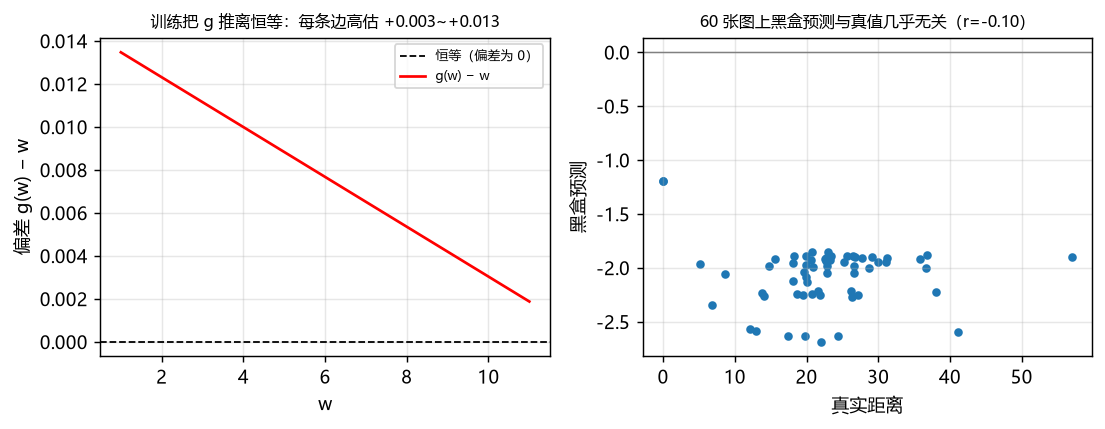
\includegraphics[width=0.70\textwidth]{fail_g_bias.png}
\caption{左：训练后的边权变换与恒等的偏差 $g(w)-w$，在 $w\in[1,10]$ 上为 $+0.003\sim+0.013$。右：黑盒 L2 在 60 张测试图上的预测——横轴是真值（$0$–$60$），纵轴是预测，全部挤在负值附近。}
\label{fig:gbias}
\end{figure}

\subsection{鲁棒性：不敏感不等于稳健}\label{sec:robust-exp}

\begin{table}[H]
\centering
\caption{扰动下的 MAE（权重噪声 20\% / 删边 10\%；另列任务本身的变化量）}
\label{tab:robustexp}
\begin{tabular}{lccc}
\toprule
模型 & 干净 & 权重噪声后 & 删边后 \\
\midrule
L0 & $5.8\times10^{-7}$ & $5.8\times10^{-7}$ & $5.8\times10^{-7}$ \\
L1 & 0.035 & 0.035 & 0.036 \\
L2 & 22.93 & 22.83 & 24.43 \\
\midrule
任务本身的变化 & --- & 5.8\% & 9.6\% \\
\bottomrule
\end{tabular}
\end{table}

表~\ref{tab:robustexp} 里有两件事值得说。

第一，L0 的误差在扰动下仍然是浮点零——它本来就是在扰动后的图上重新算，这正是“白盒的鲁棒性等于可证明性”的意思。

第二，L2 的误差从 22.93 变成 22.83，几乎不动。\textbf{这不能读成“稳健”}：它的误差已经接近常数预测器的水平，扰动改变不了它。
把它当优点写进结论，是这类比较里最典型的误读。真正的稳健应该是“误差小且随扰动变化可控”，而 L2 两条都不满足。

规模外推上，L1 从 0.024 升到 0.041（仍是 1\% 量级），L2 从 11.77 升到 19.54，L0 恒为 0。

\subsection{可解释性：保真度会被常数预测器骗过}\label{sec:interp}

先看一个“漂亮”的数字：L2 的 Fidelity$^+$ 是 \textbf{0.978}——只保留它的 top-$k$ 解释边，预测几乎不变，看起来解释得非常好。
但同一个模型在解释实验的 28 张图上，预测与真值的相关系数只有 \textbf{0.13}、标准差仅为真值的 \textbf{2.9\%}；在失败案例用的 60 张图上相关系数是 $\mathbf{-0.10}$、负预测比例 100\%。
一个几乎不看输入的模型，删掉任何边它的预测都不会怎么变——保真度自然高。\textbf{高保真度在这里度量的是模型的迟钝，不是解释的质量。}

因此我们把跨臂比较换成三个与任务绑定的指标（表~\ref{tab:interp}）。

\begin{table}[H]
\centering
\caption{解释与任务的关系（28/30 张图；2 张因 $s=t$ 退化被丢弃）}
\label{tab:interp}
\small
\setlength{\tabcolsep}{4pt}
\begin{tabular}{lccccc}
\toprule
模型 & 解释边精度 & 成路率 & 放权 $\Delta$ & Fid$^+$ & 随机 Fid$^+$ \\
\midrule
L0 & 1.00 & 100\% & 3.41 & 1.000 & $-4452$ \\
L1 & 1.00 & 100\% & 3.41 & 1.000 & $-4446$ \\
L2 & 0.50 & 11\% & 4.17 & 0.978 & 0.29 \\
\bottomrule
\end{tabular}
\end{table}

其中“成路率”指解释边能连成一条 $s$--$t$ 路的样本比例，“放权 $\Delta$”指把这些边的权重放大 10 倍后\emph{真实}最短距离的相对变化。

结论要分两句话说。\textbf{其一}，黑盒的梯度显著性对\emph{模型}是忠实的：它的 Fidelity$^+$（0.978）远高于随机选 $k$ 条边（0.29），说明它确实找到了对模型输出重要的边。
\textbf{其二}，它在“解释边精度”与“成路率”两项上与任务脱节：只有 11\% 的样本能把这些边连成一条 $s$--$t$ 路，精度 0.50（随机基线 0.00），而结构臂是 100\% 与 1.00。

还有一条观察，我原本想写成“黑盒解释无关紧要”，被数据否掉了：把解释边权重放大 10 倍，黑盒的真实距离变化是 4.17，比结构臂的 3.41 还大。
原因是显著性在并列分数上按边号取 top-$k$，选中的多是与源点相连的边，它们恰好落在最短路的头几跳上。\textbf{“有影响”不等于“解释对了”}——这条必须写进来，否则结论就过头了。

\subsection{失败案例}\label{sec:fail}

只看最大误差样本容易变成挑樱桃，所以先给分布：60 张测试图上，L2 的中位误差 24.56、90 分位 33.61、\textbf{负预测比例 100\%}（预测区间 $[-2.69,-1.19]$），预测与真值的相关系数 $r=-0.10$；
同一批图上，把 L1 的\emph{参数}只用 8 层推理（与 L2 同深度），中位误差 0.04、均值 0.391、不可达比例 2\%。

\begin{figure}[H]
\centering
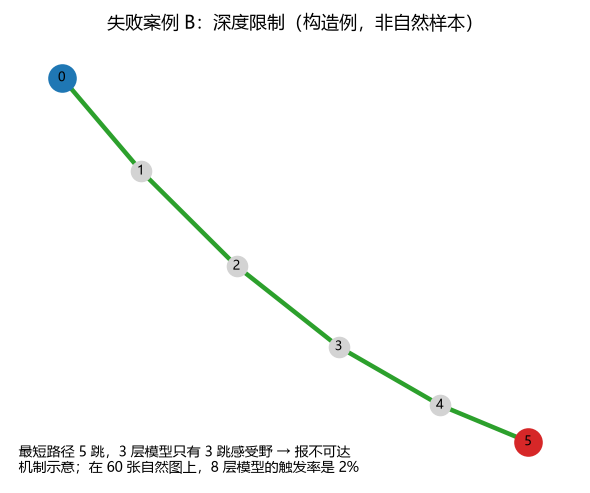
\includegraphics[width=0.40\textwidth]{fail_depth_limit.png}
\caption{失败案例：最短路径 5 跳，而 3 层恒等 min-sum 只有 5 跳以内的 3 跳感受野，于是报“不可达”。这是\emph{构造例}（既不是 L1 也不是 L2），用于演示机制；在 60 张自然图上，8 层模型的触发率是 2\%。}
\label{fig:depthfail}
\end{figure}

三类失败对应三种机制：
\begin{enumerate}[leftmargin=1.8em]
\item \textbf{黑盒没有值域约束}：它输出的距离可以为负，而距离在定义上非负。这不是某个样本的异常，是整批图上的常态。
\item \textbf{结构臂受深度限制}（图~\ref{fig:depthfail}）：$K$ 层只能看 $K$ 跳，超出即不可达。这是命题~\ref{prop:depth} 的实验版本，\emph{训练救不了}。
\item \textbf{训练的微小偏差被迭代放大}（图~\ref{fig:gbias} 左）：0.15\% 的参数偏差，经过 128 轮变成 0.024 的误差。
\end{enumerate}

需要说明口径：本节用 60 张图（种子 3000--3059），第~\ref{sec:acc}~节的 $11.77$ 用 40 张（3000--3039），两个“最坏误差”（50.6 与 58.9）不可直接并列。


\section{讨论}\label{sec:discussion}

\subsection{三轴不是一条权衡曲线}

题目把问题写成“可解释性 vs. 性能”，隐含了一个单维权衡：解释性换来性能，或者反过来。
本文的实验不支持这个图景。在最短路这个任务上，白盒在三个轴上\emph{同时}占优：

\begin{table}[H]
\centering
\caption{三轴上的对照（各行的图集不同，末列注明 $n$；L1 为 128 轮，L2 为 8 层）}
\label{tab:three}
\small
\setlength{\tabcolsep}{4pt}
\begin{tabular}{llllc}
\toprule
轴 & L0 / L1（白盒） & L2（黑盒） & 口径 & $n$ \\
\midrule
准确率 & $\sim10^{-6}$ / $0.024$ & 11.77（中位 14.92，最好 2.19） & 同分布 ER & 40 \\
鲁棒性 & $\sim10^{-6}$ / $0.035$ & 22.93 $\to$ 22.83 & 权重噪声 20\% & 30 \\
可解释性 & 精度 1.00，成路率 100\% & 精度 0.50，成路率 11\% & 同预算 $k$ & 28 \\
\bottomrule
\end{tabular}
\end{table}

这张表能说与不能说要分清。\textbf{能说}：在“允许结构臂迭代到收敛（128 轮）”这个设定下，白盒在三轴上占优。
\textbf{不能说}：白盒在任何设定下都占优——表~\ref{tab:same} 已经给出反例：同深度（8 层）时，结构臂在 SBM 上反而更差（35.38 对 28.76，$p<0.001$），在网格与规模外推上不显著（$p=0.095$）。
换句话说，白盒的胜势有一半来自“它本来就不需要层数这个约束”，而不是“结构比黑盒更会学”。

关于计算开销，本文没有做公平的对比，因此不放进表里：白盒真正的成本是跑一次 Dijkstra（$n=800$ 时 4.1\,ms，见第~\ref{sec:white}~节），而 L0 之所以要跑 128 轮，是因为我们\emph{把它写成了模型}；真实场景里没有人会那样用白盒。

所以正确的问题不是“要解释还是要性能”，而是：\textbf{你知不知道算法}。知道，就把它写进结构里，三轴一起赢；不知道，才需要在解释与性能之间做取舍。

\subsection{可验证性缺口}

本文建议用一个更锋利的量来替代“可解释性”这个模糊的词：\textbf{误差有没有上界}。

白盒的误差是零，而且扰动之后的新答案落在可计算的区间里（命题~\ref{prop:mono}--\ref{prop:bound}）。
黑盒的误差没有上界：在本文的设定里，它可以输出负距离——把真值约 57 的一对点算成 $-1.9$——而没有任何机制阻止它这么做。
模型越“黑”，我们能对它的输出说的话就越少——这不是精度问题，是\emph{可验证性}问题。

这也解释了为什么 L1 那个 0.15\% 的参数偏差值得单独讨论：在一个迭代算法里，“几乎正确”不是一个稳定的状态，误差会被迭代放大。
白盒的正确性是\emph{结构性}的（恒等映射写死在结构里），黑盒的正确性是\emph{近似性}的，两者在单步上可能看不出差别，但在 128 步之后就分开了。

\subsection{结论的边界}\label{sec:limits}

这一节的每一条都是对本文结论的削弱，但必须写。

\begin{enumerate}[leftmargin=1.8em]
\item \textbf{基线没有调到最好。}L2 的 6/8 个种子塌缩成常数预测，说明这个 mean-pool 基线训练得并不好。它最好的一次是 1.90，仍比 L1 差两个数量级，但“GNN 学不了最短路”这个更强的结论，本文的数据\emph{不支持}。能支持的只是：在这个未调好的基线上，结构先验带来 2--3 个数量级的差距。
\item \textbf{参数量不对称。}L1 有 2 个参数，L2 有 $104{,}321$ 个。这是刻意的：结构对齐的意义就是“用先验换样本”，硬把 L1 扩到同等参数量等于人为削弱它。但读者应当把参数量摆在心里看表。
\item \textbf{迭代预算不对称。}L1 在推理时跑 128 轮（迭代到收敛），L2 只有训练时的 8 层。这不是黑盒的固有属性——如果把 L2 的每层参数共享，它也可以跑 128 轮——而是我们的设计选择。因此 L1 与 L2 的比较是联合比较，不是受控消融。
\item \textbf{任务是被刻意选的。}最短路有精确解、有已知算法、真值可精确计算。这恰好是白盒的主场。换成“给定部分观测预测用户会走哪条路”这类任务，白盒的先验就不再完整，权衡曲线会重新出现。
\item \textbf{可解释性指标本身有陷阱。}本文用了一个反例说明 Fidelity$^+$ 会被常数预测器骗过。这说明“可解释性”没有公认的单一度量，任何单一数字都可能被刷。我们用三个与任务绑定的指标来交叉验证，但这仍不是终局。
\item \textbf{只跑了一组超参。}L1 的训练只用了 40 轮、学习率 $10^{-2}$、固定初始化，没有做超参扫描，也没有画 $(a,b)$ 的损失面。因此“训练停在 0.9988 而不是 1”这个观察，不能排除“换一组设置就能收敛”。我们保留这个观察，但不把它上升为“学习必然失败”的结论。
\item \textbf{有一篇直接的反例必须提。}Nerem 等人~\cite{nerem2025ood} 证明：带合适正则的 GNN 可以\emph{精确}实现 Bellman-Ford，并在规模上外推。这与本文 L0 的结论一致（结构对了就精确），但同时说明本文 L2 的失败更像“基线没调好”，而不是“GNN 学不会最短路”。本文的强结论只到“未调好的 mean-pool 基线做不到”为止。
\end{enumerate}

\subsection{什么时候黑盒才值得}

按本文的逻辑，黑盒的价值应当出现在“算法未知或不可写”的地方：
目标函数没有多项式算法、输入带有感知噪声（图像、文本、传感器）、或者人自己也说不清规则、只能给例子。
在这些场合，白盒根本没有可写的东西，讨论“误差有没有界”也就无从谈起——此时黑盒是唯一选择，可解释性则退化为一种\emph{审计}工具：不是去证明它对，而是去发现它在什么情况下会错。

反过来，如果一个任务已经有精确算法，而模型的作用只是加速或近似它，那么最划算的做法不是“用 GNN 学这个算法”，而是“把这个算法写进结构里，让学习只去补它缺的那部分”。
本文的 L0 就是前者的极端情形：当结构已经完整时，学习不但没有增益，还会破坏它。

\section{结论}\label{sec:conclusion}

本文以单源最短路为载体，把图算法的“白盒”与“黑盒”放进同一个任务、同一批图、同一套指标里做对照，得到三条结论。

\begin{enumerate}[leftmargin=1.8em]
\item \textbf{结构上，二者可以精确对应。} $k$ 层 min-sum 消息传递与同步 Bellman-Ford 的第 $k$ 轮逐点等价（定理~\ref{thm:equiv}）。
这条等价把“深度”与“边数”绑定在一起，从而给出一个构造性的深度下界：$L$ 层模型在两张 $L$ 跳计算图同构、真值不同的图上必然出错，且与训练无关（命题~\ref{prop:depth}）。
\item \textbf{白盒的鲁棒性是可证明性。} 删边单调、非树边不变、单边删除有可计算上界（命题~\ref{prop:mono}--\ref{prop:bound}），500 例验证零违反。
黑盒没有对应的命题，只能给经验分布；而在本文的实验里，它的“不敏感”其实是“没在算”。
\item \textbf{训练未必有益。} 未训练的恒等 min-sum 误差 $\sim10^{-6}$，训练 2 个参数之后反而退化到 $0.024$。
原因不是优化没做好，而是“用有限深度的监督去学一个无限迭代的算法”本身有结构性困难：损失谷底很平，学到的参数离精确解只差 0.15\%，但迭代会把这个偏差放大。
\end{enumerate}

由此得到的判断是：在最短路这类\emph{算法已知}的问题上，“可解释性 vs. 性能”的权衡曲线并不存在——白盒在准确率、鲁棒性、可解释性、计算开销四个维度上同时占优。
权衡只在算法未知时才出现；而那时，可解释性的作用不是“证明它对”，而是“发现它什么时候会错”。

\subsection*{局限与后续工作}

本文的局限已在第~\ref{sec:limits}~节逐条列出，其中最重要的两条是：黑盒基线没有调到最好（6/8 个种子塌缩），以及 L1 与 L2 的迭代预算不对称。
后续工作有三个方向：
（1）把黑盒换成权重共享的结构，让它也能迭代到收敛，从而消掉迭代预算这个不对称；
（2）把“可验证性缺口”形式化成一个可计算量（例如输出值的可达区间），而不只是一个概念；
（3）把任务从“有精确解”扩展到“有近似算法”（如旅行商），看看权衡曲线是否重新出现。

\subsection*{复现}

全部实验在纯 CPU 上完成，依赖仅为 \texttt{numpy}、\texttt{networkx}、\texttt{matplotlib} 与 \texttt{torch}，不含任何外部数据集。
仓库结构、运行命令与结果文件见 \texttt{README.md}；每个实验都有对应的验收脚本，并配有“桩实现必须失败”的负控制。


{\small
\bibliographystyle{plain}
\bibliography{refs}
}

\end{document}




